% !TEX TS-program = pdflatex
% !TeX program = pdflatex
% !TEX encoding = UTF-8
% !TeX spellcheck = en_US

\documentclass{../extra/aakpract/aakpract}

\usepackage{listings}
\usepackage{makecell}

\usetikzlibrary{shapes.geometric}

\settitle{Parsing}
\setversion{Tutorial}
\setyear{2025-2026}
\setauthor{Dr. Abdelkrime Aries}
\setfooter{Tutorial: Parsing}

\begin{document}
	
	\maketitle
	
	\begin{center}
		\begin{minipage}{0.85\textwidth}
			\small\itshape
			This tutorial introduces the main concepts behind sequence labeling in NLP through the example of Part-of-Speech (PoS) tagging. 
			Sequence labeling consists in assigning a label to each token in a sentence while accounting for contextual dependencies between words and labels.
			
			\vspace{6pt}
			The tutorial reviews several modeling approaches, including generative models such as Hidden Markov Models (HMMs), discriminative models like Maximum Entropy Markov Models (MEMMs), and neural architectures based on recurrent neural networks (RNNs) and Transformers. 
			Through analytical questions and decoding exercises, students explore how these models represent contextual information, model label dependencies, and predict the most probable sequence of tags.
			
		\end{minipage}
	\end{center}
	
	\section{Quizzes}
	
	\subsection{Midterm 2024/2025 (Modified)}
	
	Select the statements about text parsing that are correct. 
	
	\begin{longtable}{|p{.95\textwidth}|}
		\hline 
		\Square\ Arc-standard parsing identifies dependency relations incrementally, as soon as possible.\\
		\Square\ Chunking is both a sequence labeling application and a simple text parsing method.\\
		\Square\ A well trained Graph-based parser would give the same result as a well trained Transition-based parsing on a sentence from the training dataset.  \\
		\Square\ A well trained Graph-based parser would give the same result as a well trained Transition-based parsing on a sentence from the test dataset. \\
		\Square\ CKY is a bottom-up parsing algorithm parsing algorithm based on dynamic programming,  which uses the Chomsky normal form as a precondition. \\
		\Square\ CKY has exponential time complexity in the length of the input.\\
		\Square\ Dependency trees must always have multiple roots to handle compound sentences.\\
		\hline
	\end{longtable}
	
	\subsection{Midterm 2023/2024 (Modified)}
	
	Among these statements about text parsing, select the correct ones:
	
	\begin{longtable}{|p{.95\textwidth}|}
		\hline 
		\Square\ Arc-standard does not need a REDUCE transition because it allows a non-empty stack final configuration.\\
		\Square\ Using PoS tagging for constituency parsing results in fewer grammar production rules.\\
		\Square\ Before Graph-based parsing, we can apply a preprocessing step to reduce the graph size.\\
		\Square\ Transition-based parsing can be used for constituency parsing with one pass.\\
		\Square\ Given $N$ words, the initial graph in Graph-based parsing has $N^2$ arcs.\\
		\Square\ Arc-eager parsing tends to find relations earlier than Arc-standard.\\
		\Square\ CKY algorithm can be modified to parse unit productions.\\
		\Square\ CKY algorithm can be used for dependency parsing.\\
		\Square\ Dependency formalism allows ternary relations.\\
		\hline
	\end{longtable}
	
	\subsection{Midterm 2022/2023 (Modified)}
	
	Among these statements about text parsing, select the correct ones:
	
	\begin{longtable}{|p{.95\textwidth}|}
		\hline 
		\Square\ CFG-based parsing generates a tree which has PoS as leaf nodes. \\
		\Square\ Dependency parsing also generates a tree structure. \\	
		\Square\ Dependency formalism is based on syntactic functions. \\
		\Square\ CKY's original algorithm uses only CFGs in Chomsky normal form. \\
		\Square\ CKY's original algorithm always generates a tree similar to those defined by syntacticians. \\
		\Square\ Probabilistic CKY is trained on the same dataset as the plain CKY algorithm. \\
		\Square\ Transition-based parsing is trained using an unsupervised method. \\
		\Square\ Arc-standard finds dependencies earlier than Arc-eager. \\
		\Square\ Graph-based parsing is mainly used for constituency parsing.\\
		\hline
	\end{longtable}
	
	
	
	\section{Constituency parsing}
	
%	\subsection{Grammars}
%	
%	Here is a grammar (phrases and lexicon):
%	
%	\begin{tabular}{|lllll|}
%		\hline
%		S \textrightarrow\ NP VP & NP \textrightarrow\ DET N && DET \textrightarrow\ le \textbar\  la & NN \textrightarrow\ Toma \textbar\  Jerry \\
%		NP \textrightarrow\ NN & VP \textrightarrow\ VT NP &&  N \textrightarrow\  souris \textbar\  chat \textbar\  fromage \textbar\  maison & P \textrightarrow\ de\\
%		VP \textrightarrow\ VI & PP \textrightarrow\ P NP && VT \textrightarrow\ mange \textbar\  vole & VI \textrightarrow\ dort \textbar\  sort\\
%		\hline
%	\end{tabular}
%	
%	\begin{enumerate}
%		\item Add rules to generate the following sentences: (1) Le chat dors (2) La souris mange le fromage (3) Tom vole le fromage de la souris (4) Tom sort de la maison.
%		\item Why are proper nouns separated from the set of nouns?
%		\item We want to be able to generate the sentence: Nora vole le fromage du chat. The grammar should not generate a sentence like: Jerry vole la fromage de le chat. What rules should be added and removed? (In French: "de le" becomes "du".)
%	\end{enumerate}
	
	\subsection{Midterm 2024/2025 (Modified)}
	
%	\begin{center}
%		\begin{tabular}{|p{.15\textwidth}|p{.3\textwidth}|p{.3\textwidth}|p{.15\textwidth}|}
%			\hline
%			S → VP \textbar\ NP VP &
%			NP →PR \textbar\ NN \textbar\ DT NN
%			\textbar\ JJ NN  \textbar\ DT JJ NN &
%			NN → Eid \textbar\ prayers \textbar\ hope \textbar\ wish&
%			DT → a \textbar\ the \\
%			
%			
%			AP → JJ CC AP \textbar\ JJ &
%			VP → VB \textbar\ VB NP \textbar\ VB VB
%			\textbar\ VB SBAR \textbar\ VB AP
%			\textbar\ VB NP NP &
%			VB → wish \textbar\ hope \textbar\ be \textbar\ have \textbar\ are 
%			\textbar\ answered \textbar\ blessed &
%			CC → and \textbar\ or \\
%			
%			SBAR → S &&
%			JJ → blessed \textbar\ happy \textbar\ peaceful 
%			\textbar\ joyful &
%			PR → I \textbar\ you 
%			\textbar\ your \\
%			\hline
%		\end{tabular}
%	\end{center}
	
	\begin{enumerate}
		\item Draw two possible constituency parse trees for the ambiguous sentence ``\textbf{I wish you blessed Eid}'' using the unmodified grammar on the left. 
		Then, explain which parse is more probable and why, without computing exact probabilities (non-existent rules are assumed to have a small probability).
		
		\item Complete the modified CKY parsing using the Chomsky Normal Form (CNF) transformation and the CKY table provided below.
		In this version, unary rules are resolved within the same cell by adding a tuple of the form (phrase type, index of the production in the same cell).
		
		\item Only ditransitive verbs can take two noun phrase arguments, and in our lexicon, only ``\textbf{wish}'' satisfies this condition. 
		Moreover, only clause-taking verbs can be followed by an SBAR; in our lexicon, these are ``\textbf{wish}'' and ``\textbf{hope}''. 
		Based on this information, identify which grammar rules should be removed or added to prevent ungrammatical sentences such as ``\textbf{I have you a blessed Eid}'' and ``\textbf{I have your prayers are answered}''.
	\end{enumerate}
	
	
	\begin{center}
		\small
	\begin{tabular}{p{6cm}|c|c|c|c|c|}
		\cline{2-6}
		&\multicolumn{5}{|l|}{NP → DT JJ NN \textrightarrow\ NP → DT JNP ; JNP → JJ NN}\\
		&\multicolumn{5}{|l|}{VP → VB NP NP \textrightarrow\ VP → VB NP2 ; NP2 → NP NP}\\
		\cline{2-6}
		&I & wish & you & blessed & Eid \\
		\cline{2-6}
		&
		\makecell{(PR, 0, 0, 0) \\ (NP, 1)}
		&
		C[1, 2] = ?
		&
		C[1, 3] = ?
		&
		\makecell{(S, 1, 2, 1) \\ (SBAR, 1)}
		&
		\makecell{(S, 1, 2, 1) \\ (S, 1, 2, 2) \\ (SBAR, 1) \\ (SBAR, 2)}
		\\
		\cline{2-6}
		\multicolumn{2}{l|}{\makecell[l]{
				\\ \\ \\ \\
				S → VP \textbar\ NP VP \\ AP → JJ CC AP \textbar\ JJ
				}}
		&
		\makecell{(VB, 0, 0, 0) \\ (NN, 0, 0, 0) \\ (VP, 1) \\ (NP, 2) \\ (S, 3) \\ (SBAR, 5)}
		&
		C[2, 3] = ?
		&
		\makecell{(VP, 2, 1, 2) \\ (S, 1) \\ (SBAR, 2)}
		&
		C[2, 5] = ?
		\\
		\cline{3-6}
		\multicolumn{3}{l|}{\makecell[l]{
				SBAR → S\\
				NP →PR \textbar\ NN \textbar\ DT NN \textbar\ JJ NN  \textbar\ DT JJ NN
		}}
		&
		\makecell{(PR, 0, 0, 0) \\ (NP, 1)}
		&
		\makecell{(S, 3, 2, 3) \\ (SBAR, 1)}
		&
		C[3, 5] = ?
		\\
		\cline{4-6}
		\multicolumn{4}{l|}{\makecell[l]{
				VP → VB \textbar\ VB NP \textbar\ VB VB \textbar\ VB SBAR \textbar\ VB AP \textbar\ VB NP NP \\
				NN → Eid \textbar\ prayers \textbar\ hope \textbar\ wish \\
				VB → wish \textbar\ hope \textbar\ be \textbar\ have \textbar\ are \textbar\ answered \textbar\ blessed \\
				JJ → blessed \textbar\ happy \textbar\ peaceful \textbar\ joyful \\
				DT → a \textbar\ the 
		}}
		&
		\makecell{(VB, 0, 0, 0) \\ (JJ, 0, 0, 0) \\ (VP, 1) \\ (S, 3) \\ (SBAR, 5)}
		&
		C[4, 5] = ?
		\\
		\cline{5-6}
		\multicolumn{5}{l|}{\makecell[l]{CC → and \textbar\ or \\
				PR → I \textbar\ you \textbar\ your}}
		&
		\makecell{(NN, 0, 0, 0) \\ (NP, 1)}
		\\
		\cline{6-6}
	\end{tabular}
	\end{center}
	
	\subsection{Midterm 2023/2024 (Modified)}
	
	\begin{center}
		\begin{tabular}{|llll|}
		\hline
		S  → NP  VP \textbar\ VP &
		NP → P \textbar\ D N \textbar\ N &
		P → you \textbar\ they &          
		D → this \textbar\ these \\
		
		& VP → V NP &
		V → light \textbar\ fish &
		N → light \textbar\ fish \\
		\hline
		\end{tabular}
	\end{center}
	
	Draw the CKY analysis table T handling unitary productions.
	The list in each cell is enriched with unit productions of the form (PoS, position in the same list).
	Then draw the corresponding parse tree.
	The sentence to analyze is "\textbf{these fish light light}".
	
	\begin{center}
		\begin{tabular}{|l|}
			\hline
			T[1, 1] = [(D, 0, 0, 0)]; T[1, 2] = [(NP, 1, 1, 2)];  T[1, 3] = []; T[2, 2] = [(V, 0, 0, 0), (N, 0, 0, 0), (NP, 2)]\\
			\hline
		\end{tabular}
	\end{center}
	
	\subsection{Midterm 2022/2023 (Modified)}
	
	\begin{enumerate}
		\item Given the following grammar:
	\begin{center}
		\begin{tabular}{|llll|}
			\hline
			S → NP  VP & VP → V NP & P → I $|$ You & V → light $|$ torch $|$ house \\
			& NP → P $|$ D N & D → the & N → light $|$ torch $|$ house \\
			\hline
		\end{tabular}
	\end{center}
	
	Complete the following CKY analysis.
	\begin{center}\small
		\begin{tabular}{|p{2cm}|p{2cm}|p{2cm}|p{2cm}|}
			\hline
			You & light & the & house \\
			\hline
			(NP, 0, 0, 0) &&& \\
			\hline
			\multicolumn{1}{l|}{} & (V, 0, 0, 0) \newline (N, 0, 0, 0) & --- & \\
			\cline{2-4}
			\multicolumn{2}{l|}{} & (D, 0, 0, 0) & (NP, 3, 1, 2) \\
			\cline{3-4}
			\multicolumn{3}{l|}{} & \\
			\cline{4-4}
		\end{tabular}
	\end{center}
	
	\item Given the following treebank:
	\begin{center}
		\begin{tabular}{|lll|}
			\hline
			I/\textsubscript{P} light/\textsubscript{V} the/\textsubscript{D} torch/\textsubscript{N} &
			You/\textsubscript{P} torch/\textsubscript{V} the/\textsubscript{D} house/\textsubscript{N} &
			I/\textsubscript{P} house/\textsubscript{V} the/\textsubscript{D} light/\textsubscript{N} \\
			\hline
		\end{tabular}
	\end{center}
	Calculate \textbf{P(NP → D N)} using the original grammar without smoothing.
	
	\item Complete the following Chu-Liu/Edmonds parsing.
	Consider all vertices at once, rather than one at a time.
	Draw two graphs derived from the following one (two steps).
	Cycles take precedence.
	For simplicity, assume that some arcs were removed during a preprocessing step.
	
	\begin{center}
		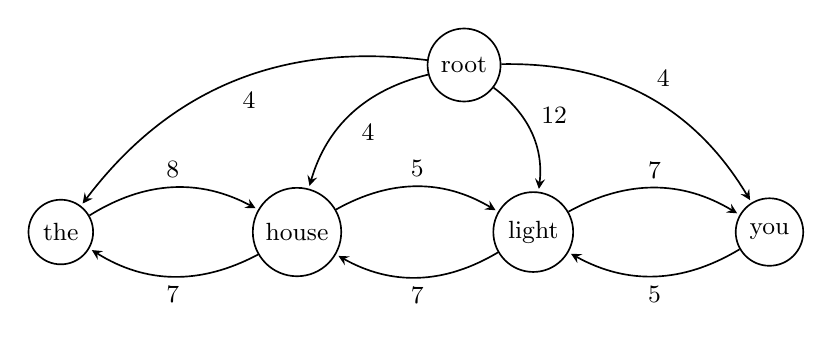
\begin{tikzpicture}[
			> = stealth, % arrow head style
			shorten > = 1pt, % don't touch arrow head to node
			auto,
			node distance = 3cm, % distance between nodes
			semithick, % line style
			font=\small
			]
			
			\tikzstyle{every state}=[
			draw = black,
			thick,
			fill = white,
			minimum size = 4mm
			]
			
			\node[circle,draw] (root) {root};
			\node[circle,draw] (house) [below left of=root] {house};
			\node[circle,draw] (the) [left of=house] {the};
			\node[circle,draw] (light) [right of=house] {light};
			\node[circle,draw] (you) [right of=light] {you};
			
			\path[->] 	
			(root) 	edge [bend right] node {4} (the)
					edge [bend right] node {4} (house)
					edge [bend left] node {12} (light)
					edge [bend left] node {4} (you)
			(the) 	edge [bend left] node {8} (house)
			(house)	edge [bend left] node {7} (the)
					edge [bend left] node {5} (light)        
			(light)	edge [bend left] node {7} (house)
					edge [bend left] node {7} (you) 
			(you)	edge [bend left] node {5} (light)
			;
		\end{tikzpicture}
	\end{center}
	
	\end{enumerate}
	
	\subsection{Midterm 2021/2022 (Extended version)}
	
	\begin{enumerate}
		
		\item Consider the following grammar (phrase rules and lexicon):
		
		\begin{tabular}{|lllll|}
			\hline
			S \textrightarrow\ NP VP & NP \textrightarrow\ AJ NM $|$ NM $|$ PN & AJ \textrightarrow\ small $|$ big  & VB \textrightarrow\ fish $|$ like $|$ swim &  \\
			PP \textrightarrow\ PR NP & VP \textrightarrow\ VB NP $|$ VB PP & NM \textrightarrow\ fish $|$ ducks & PR \textrightarrow\ like & PN \textrightarrow\ I \\
			\hline
		\end{tabular}
		
		Analyze the following sentences using CKY and draw their parse trees:
		``\textbf{big ducks like small fish}'', ``\textbf{I fish like big ducks}'', and ``\textbf{I swim like fish swim}''.
		
		\item Here is a treebank containing four sentences in which each word is annotated with its grammatical category:
		
		\begin{tabular}{|lll|}
			\hline
			I/PN fish/VB small/AJ fish/NM &&
			I/PN swim/VB like/PR fish/NM\\
			ducks/NM swim/VB &&
			I/PN like/VB big/AJ fish/NM \\
			\hline
		\end{tabular}
		
		\begin{enumerate}
			\item Calculate the probability of each grammar rule.
			\item Analyze the sentences using the probabilistic CKY algorithm.
		\end{enumerate}
		
	\end{enumerate}
	
	\section{Dependency parsing (Transition)} 
	
	\subsection{Midterm 2024/2025 (Modified)}
	
	The following dependency labels are used: \textbf{det}, \textbf{sub}, \textbf{obj}, \textbf{iobj}, \textbf{mod}, and \textbf{other}.
	\begin{enumerate}
		\item Complete the next 3 rows of the following Arc-eager parsing table to generate the parse tree shown on the right.\\
		\begin{tabular}{|l|l|l|l|ll}
			\cline{1-4}
			$\sigma$(stack) &
			$\beta$(buffer) &
			Action &
			new arc &
			&
			\multirow{3}{*}{
			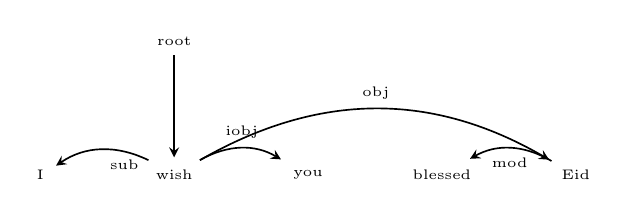
\begin{tikzpicture}[
				> = stealth, % arrow head style
				shorten > = 1pt, % don't touch arrow head to node
				auto,
				node distance = 1.7cm, % distance between nodes
				semithick, % line style
				font=\tiny
				]
				
				\tikzstyle{every state}=[
				draw = black,
				thick,
				fill = white,
%				minimum size = 4mm
				]
				
				\node[] (root) {root};
				\node[] (wish) [below of=root] {wish};
				\node[] (i) [left of=wish] {I};
				\node[] (you) [right of=wish] {you};
				\node[] (blessed) [right of=you] {blessed};
				\node[] (eid) [right of=blessed] {Eid};
				
				\path[->] 	
				(root) 	edge [] (wish)
				(wish) 	edge [bend right] node {sub} (i)
						edge [bend left] node {iobj} (you)
						edge [bend left] node {obj} (eid)        
				(eid)	edge [bend right] node {mod} (blessed)
				;
			\end{tikzpicture}
			}
			\\
			\cline{1-4}
			
			[ROOT] &
			I wish you blessed Eid &
			SHIFT &
			/ &&\\
			\cline{1-4}
			\multicolumn{6}{c}{}\\
		\end{tabular}
		
		\item For the sentence "\textbf{I wish you blessed Eid}", calculate:
		\begin{enumerate}
			\item the maximum number of classes that the Arc-eager oracle can estimate;
			\item the number of initial arcs using graph-based parsing;
			\item the number of initial arcs using graph-based parsing, knowing that det, sub, and mod are always to the left, and obj and iobj are always to the right.
		\end{enumerate}
	\end{enumerate}
	
	\subsection{Midterm 2023/2024 (Modified)}
	
	\begin{enumerate}
		\item Complete this Arc-standard parsing table where "Oracle" is the decision tree bellow. Then draw the parse tree.
		\begin{center}
			\begin{tabular}{|l|l|l|l|}
			\hline
			$\sigma$(stack) &
			$\beta$(buffer) &
			Action &
			new arc \\
			\hline
			[ROOT] &
			these fish light light &
			SHIFT &
			/ \\
			\hline
			\end{tabular}
		\end{center}
		\item Using graph-based dependency parsing, 
		\begin{enumerate}
			\item Calculate the number of initial arcs to process the sentence "\textbf{these fish light light}".
			\item Generalize for a sentence of N words.
			\item Calculate the number of initial arcs to process that sentence when we consider only arcs between words of distance equals to 1.
			\item Generalize for a sentence of N words and a maximum distance of D.
		\end{enumerate}
		
	\end{enumerate}
	
	\begin{center}
	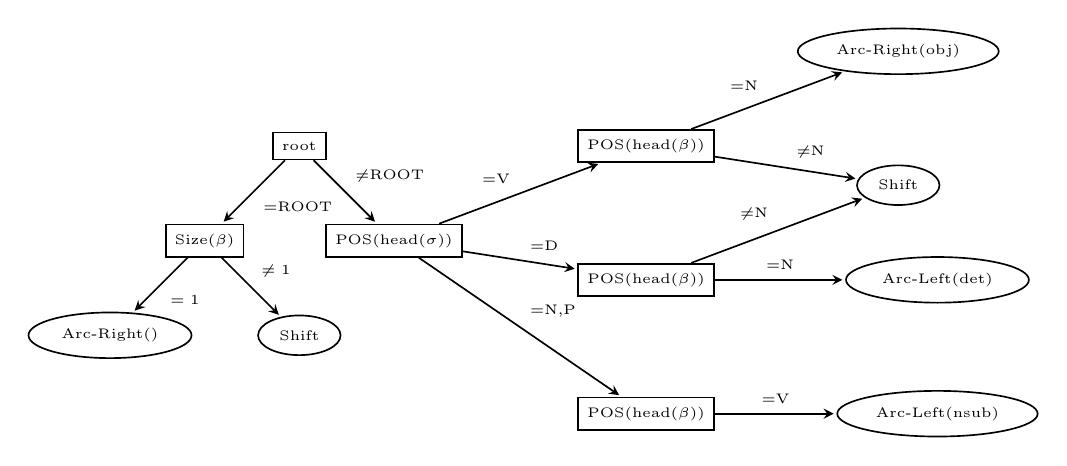
\begin{tikzpicture}[
		> = stealth, % arrow head style
		shorten > = 1pt, % don't touch arrow head to node
		auto,
		node distance = 1.7cm, % distance between nodes
		semithick, % line style
		font=\tiny
		]
		
		\tikzstyle{every state}=[
		draw = black,
		thick,
		fill = white,
		minimum size = 4mm
		]
		
		\node[rectangle, draw] (root) {root};
		\node[rectangle, draw] (pos1) [below right of=root] {POS(head($\sigma$))};
		\node[rectangle, draw] (size1) [below left of=root] {Size($\beta$)};
		\node[ellipse, draw] (shift1) [below right of=size1] {Shift};
		\node[ellipse, draw] (ar1) [below left of=size1] {Arc-Right()};
		
		\node[rectangle, draw] (pos21) [above right of=pos1, xshift=2cm] {POS(head($\beta$))};
		\node[rectangle, draw] (pos22) [below of=pos21] {POS(head($\beta$))};
		\node[rectangle, draw] (pos23) [below of=pos22] {POS(head($\beta$))};
		
		\node[ellipse, draw] (ar21) [above right of=pos21, xshift=2cm] {Arc-Right(obj)};
		\node[ellipse, draw] (shift22) [below of=ar21] {Shift};
		
		\node[ellipse, draw] (al21) [right of=pos22, xshift=2cm] {Arc-Left(det)};
		\node[ellipse, draw] (al22) [right of=pos23, xshift=2cm] {Arc-Left(nsub)};
		
		\path[->] 	
		(root) 	edge [] node {=ROOT} (size1)
				edge [] node {$\ne$ROOT} (pos1)      
		(size1)	edge [] node {$\ne1$} (shift1)
				edge [] node {$=1$} (ar1)
		(pos1)	edge [] node {=V} (pos21)
				edge [] node {=D} (pos22)
				edge [] node {=N,P} (pos23)
		(pos21)	edge [] node {=N} (ar21)
				edge [] node {$\ne$N} (shift22)
		(pos22)	edge [] node {=N} (al21)
				edge [] node {$\ne$N} (shift22)
		(pos23)	edge [] node {=V} (al22)
		;
	\end{tikzpicture}
	\end{center}
	
	\subsection{Midterm 2022/2023 (Modified)}
	
	Complete the following Arc-eager parsing table (the oracle is assumed to be well trained).
	\begin{center}
		\begin{tabular}{|c|c|c|c|}
			\hline
			$ \sigma $ (Stack) & $ \beta $ (Buffer) & Action & New arc \\
			\hline
			[ROOT] & You light the house & SHIFT & / \\
			\hline
			&  &  & light→You \\
			\hline
			[ROOT] &  &  &  \\
			\hline
			&  & SHIFT & / \\
			\hline
		\end{tabular}
	\end{center}
	
	\subsection{Midterm 2021/2022 (Extended version)}
	
	\begin{enumerate}
		\item Analyze the following sentences using a perfectly trained Arc-standard parser and draw their dependency trees:
		``\textbf{big ducks like small fish}'', ``\textbf{I fish like big ducks}'', and ``\textbf{I swim like fish swim}''.
		\item Perform the same analysis using a perfectly trained Arc-eager parser.
		\item Here is a treebank containing four sentences, where each word is annotated with its grammatical category:
		\begin{center}
			\begin{tabular}{|lll|}
				\hline
				I/\textsubscript{PN} fish/\textsubscript{VB} small/\textsubscript{AJ} fish/\textsubscript{NM} &&
				I/\textsubscript{PN} swim/\textsubscript{VB} like/\textsubscript{PR} fish/\textsubscript{NM}\\
				ducks/\textsubscript{NM} swim/\textsubscript{VB} &&
				I/\textsubscript{PN} like/\textsubscript{VB} big/\textsubscript{AJ} fish/\textsubscript{NM} \\
				\hline
			\end{tabular}
		\end{center}
		
		Train a logistic regression model that predicts the next action (3 classes) based on the word and tag features (a vector of 12 integers: 5 tags + 7 words).
		To simplify the calculation: 
		\begin{itemize}
			\item perform only 5 iterations,
			\item use normalization instead of Softmax as the activation function,
			\item use the cost function without the logarithm term.
		\end{itemize}
		
		\item Suppose we have a word encoding model as follows: $Em(w_1\dots w_n) = \frac{\sum_{i=1}^{n} Pos(w_i)}{n}$ where $Pos$ is the position of the character in the alphabet. A model $Et$ for encoding tags involves ordering the tags alphabetically and returning the order of the tag as the code. Suppose we have trained a link scoring model where $Notation((u, v)) = \frac{Et(u) - Et(v)}{1+ Em(u)*Em(v)}$. We take $Em(Root) = 0$ and $Et(Root) = 0$. Analyze the dependencies of the sentence "ducks like fish" using the graph-based method.
		
	\end{enumerate}
	
	\section{Critical Thinking}
	
	\subsection{Midterm 2024/2025 (Modified)}
	
	We aim to design an English constituency parser based on Transformer architectures. 
	
	\begin{enumerate}
		\item Propose a model architecture suitable for constituency parsing using a Transformer model: encoder-only (e.g., BERT, XLNet), decoder-only (e.g., GPT), or encoder–decoder (e.g., T5, BART). 
		Specify the chosen Transformer type, the input and output representations, the parsing strategy, and any required adaptations when using a model pretrained on standard English corpora.
		
		\item To improve model performance, consider incorporating manually designed linguistic features. 
		Propose two such features and explain how they can be integrated into the model.
		
		\item Propose a hybrid architecture for constituency parsing that combines Transformer, RNN, and CNN components. 
		Clearly describe the role of each component.
		
		\item State one advantage and one disadvantage of using Transformer-based models for constituency parsing compared to traditional methods such as probabilistic CKY.
	\end{enumerate}
	
	
\end{document}
